\section{Introduction}
\label{sec:intro}


Large language model (LLM) agents are becoming remarkably capable at real-world software engineering tasks~\citep{jimenez2024swebench,mundler2024swtbench}, thanks to their strong reasoning and tool-use abilities~\citep{yang2024swe,openhands,claudecode}.
This growing capability has significant implications for the critical domain of cybersecurity, presenting both opportunities and risks~\citep{guo2025frontieraisimpactcybersecurity}.
Therefore, it is both critical and urgent to rigorously assess AI agents' cybersecurity capabilities.
Recently, several useful cybersecurity benchmarks have been developed.
Some are based on classic capture-the-flag (CTF) challenges~\citep{cybench,shao2024nyu}, while others leverage historical vulnerabilities from real software projects~\citep{carlini2025autoadvexbench,zhu2025cve,zhang2025bountybench,lee2025sec}.
However, they suffer from two key limitations:%
\begin{enumerate}[leftmargin=*,topsep=-2pt,label=(\roman*),parsep=0pt]
    \item They are small-scale (up to 200 instances, see \cref{tab:comp}), due to relying on significant manual benchmark building effort or brittle data sources. This small scale can lead to unstable evaluations and may not capture the full range of complexities in practical cybersecurity.
    \item Their evaluation results are solely focused on static benchmark instances, making it difficult to determine how AI agents impact constantly evolving, current cybersecurity landscape.
\end{enumerate}

\begin{figure}[t]
    \centering
    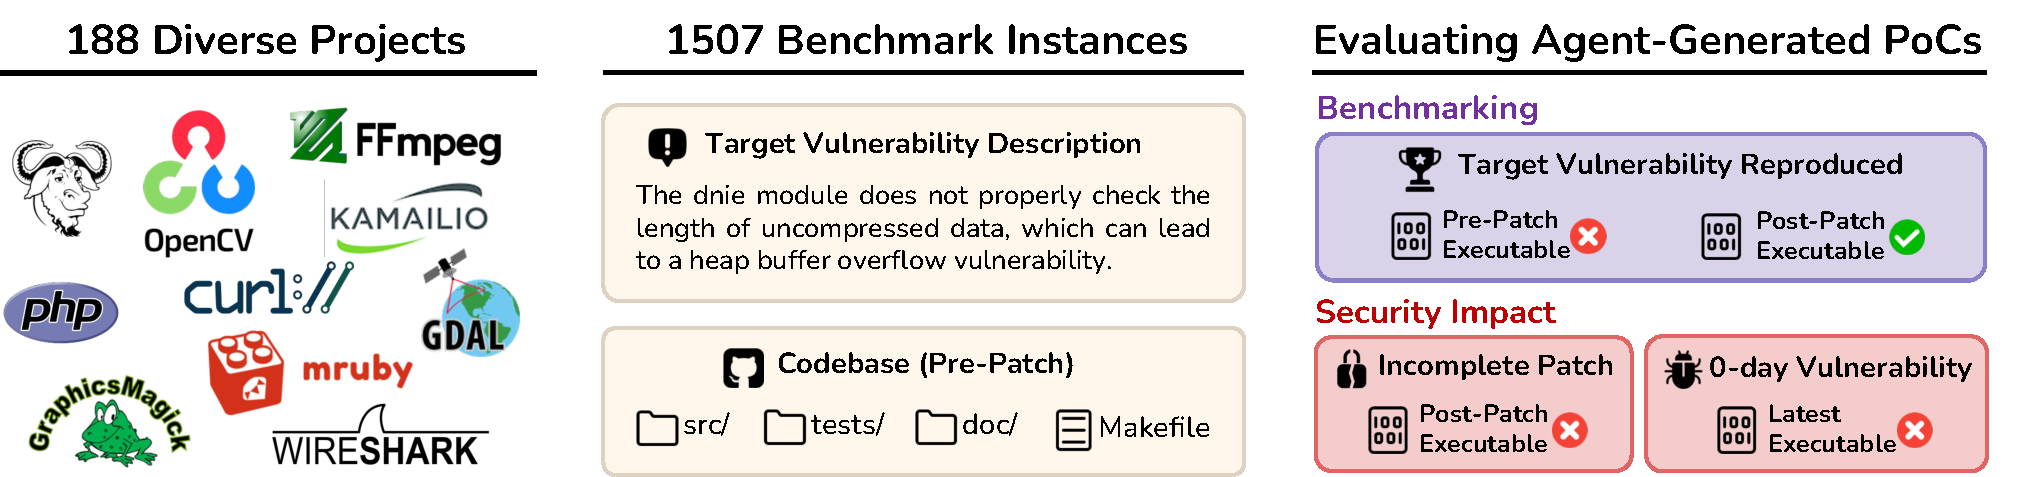
\includegraphics[width=\linewidth]{figures/overview_img.pdf}
    \vspace{-5.3mm}
    \caption{\sysname includes 1,507 instances from real-world vulnerabilities across 188 diverse projects. For benchmarking, AI agents receive vulnerability descriptions and pre-patch codebased to generate proof-of-concept (PoC) tests for vulnerability reproduction. Going a step further, \sysname creates direct security impact via detecting incomplete patches and zero-day vulnerabilities.}
    \label{fig:intro}
    \vspace{-5mm}
\end{figure}


\paragraph{\sysname: A Large-Scale, Realistic Cybersecurity Benchmark}
To address limitation (i), we introduce \sysname, a large-scale and realistic cybersecurity benchmark\footnote{\sysname has been adopted in the system cards of various frontier models for cybersecurity evaluation, such as Claude~\citep{claudeopus45,claudesonnet45,claudeopus46,claudesonnet46}, Kimi~\citep{team2026kimi}, and GLM~\citep{zeng2026glm}.}.
As illustrated in~\cref{fig:intro}, \sysname contains 1,507 benchmark instances derived from real-world vulnerabilities across 188 widely used software projects spanning diverse domains.
These vulnerabilities are sourced from OSS-Fuzz~\citep{ossfuzz}, Google's continuous fuzzing service.
We ensure the quality and timeliness of our benchmark instances through systematic automated filters and manual validation.

\sysname primarily evaluates agents on their ability to reproduce vulnerabilities, a key task in software security that often challenges even human experts~\citep{bohme2017directed,klees2018evaluating,mu2018understanding}.
As shown in \cref{fig:intro}, given a text description of a vulnerability and the associated codebase, agents must produce a proof-of-concept (PoC) test to reproduce it, i.e., to demonstrate the existence of the target vulnerability.
We rigorously validate generated PoCs by executing them on both pre-patch and post-patch versions to confirm reproduction success.
Solving \sysname requires agents to perform deep reasoning across large codebases, spanning thousands of files and millions lines of code.
They must locate relevant code sections and produce effective PoCs of diverse formats and sizes to trigger the vulnerability.
Beyond the main task, \sysname supports different difficulty levels that simulate various stages of the vulnerability lifecycle, including discovering vulnerabilities exploratively or reproducing them given additional patch information to simulate real-world one-day scenarios.
\sysname's modular, containerized design ensures reproducible, extensible, and scalable evaluation, allowing for easy assessment of future agents and integration of new benchmark instances.

\paragraph{\sysname Challenges Frontier Agents with a Ladder of Difficulty}
We conduct an extensive evaluation of four state-of-the-art agent frameworks and eleven frontier LLMs on \sysname.
Our results highlight that \sysname is a challenging benchmark that effectively differentiates these approaches based on their cybersecurity capabilities.
The best-performing combination (if no ``thinking'' mechanism is enabled) is \openhands~\citep{openhands} with \claudeiv~\citep{claudesonnet4}, which achieves only a 17.9\% success rate.
We also show that turning on ``thinking'' improves \claudeiv only slightly, but significantly for \gptv~\citep{openai_gpt5}, which jumps from a 7.7\% to a 22.0\% success rate.
Specialized software engineering models~\citep{swegym,r2egym,openhands_lm32b} exhibit poor generalization on \sysname, with $\leq$2.0\% success rates, demonstrating \sysname's complementary nature to SWE-bench~\citep{jimenez2024swebench}.
Our in-depth analysis shows that current approaches mainly solve simpler tasks requiring fewer agent execution steps and shorter PoCs.
These results indicate that \sysname's diverse and challenging tasks provide a gradual ladder of difficulty, enabling tracking current and future progress in the cybersecurity field.

\paragraph{\sysname Extends to Creating Direct, Real-World Security Impact}
Beyond benchmarking, \sysname produces a direct impact on practical security, addressing limitation (ii).
During our evaluation, we found that even when tasked with reproducing a specific vulnerability, the agents can inadvertently generate PoCs that trigger different vulnerabilities.
These unintended PoCs affect program versions where the target vulnerability has been patched, or even the latest version.
Our analysis of these PoCs reveal 17 inadequate historical patches and 10 previously unknown vulnerabilities, i.e., zero-days.
To further validate this capability, we deploy the agents for open-ended vulnerability discovery across 431 open-source projects, identifying an additional 25 unique zero-day vulnerabilities.
We have responsibly disclosed all zero-days to project maintainers, with 4 CVE assignments received and 10 vulnerabilities patched as of this writing.

\paragraph{Main Contributions}
In summary, we make the following key contributions:
\begin{itemize}[leftmargin=*,topsep=0pt,parsep=0pt]
    \item A large-scale and realistic cybersecurity benchmark with diverse and challenging benchmark instances and rigorous execution-based metrics (\cref{sec:dataset}).
    \item A comprehensive evaluation for various frontier agents and LLMs with over \$40,000 USD API credits and 1,000 H100 GPU hours, providing valuable insights into the emerging capabilities and current limitations of AI agents in cybersecurity (\cref{sec:eval}).
    \item A platform performing open-ended vulnerability discovery analysis, demonstrating the substantial practical security impact of AI agents on real-world software (\cref{sec:discovery}).
    \item The discovery and disclosure of 34 zero-days in popular open-source projects (\cref{app:discovery}).
\end{itemize}
